\documentclass[border=10pt]{standalone}
\usepackage{tikz}
\usetikzlibrary{arrows.meta, shapes, calc, positioning}

\begin{document}
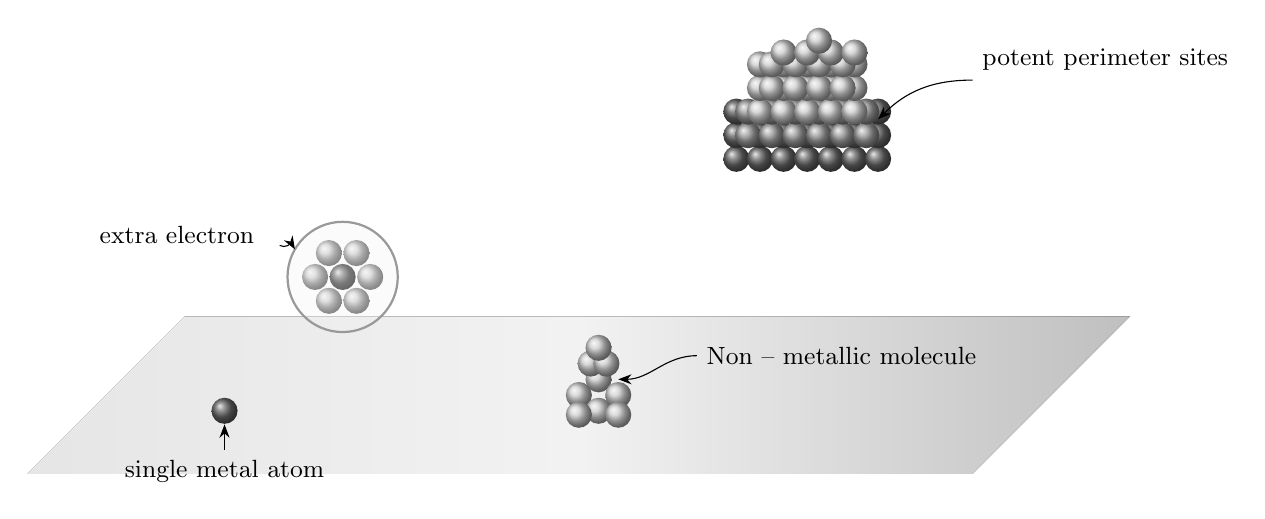
\begin{tikzpicture}[
    sphere/.style={circle, shading=ball, minimum size=0.3cm},
    metal/.style={sphere, ball color=black!60},
    light/.style={sphere, ball color=black!20},
    medium/.style={sphere, ball color=black!40}
]

% Draw the surface (parallelogram with shading)
\fill[left color=black!10, right color=black!25, middle color=black!5] 
    (0,0) -- (12,0) -- (14,2) -- (2,2) -- cycle;

% Single metal atom (bottom left)
\node[metal] (atom) at (2.5,0.8) {};
\draw (2.5,0.8) node[below=0.5cm, align=center] {\small single metal atom};
\draw[-Stealth] (2.5,0.3) -- (atom);

% Single metal atom with extra electron (left, with halo)
\node[metal] (atomElec) at (4,2.5) {};
\foreach \angle in {0,60,120,180,240,300} {
    \node[light, minimum size=0.15cm] at ($(atomElec)+(\angle:0.35)$) {};
}
\fill[black!5, opacity=0.3] (4,2.5) circle (0.7);
\draw[thick, black!40] (4,2.5) circle (0.7);
\draw (3,2.8) node[above left, align=center] {\small extra electron};
\draw[-Stealth] (3.2,2.9) to[out=-30, in=120] ($(atomElec)+(150:0.7)$);

% Non-metallic molecule (bottom center)
\begin{scope}[shift={(7,1)}]
    \node[light] at (0,0) {};
    \node[light] at (0.25,0.2) {};
    \node[light] at (0.5,0) {};
    \node[light] at (0.25,-0.2) {};
    \node[light] at (0,-0.25) {};
    \node[light] at (0.5,-0.25) {};
    \node[light] at (0.15,0.4) {};
    \node[light] at (0.35,0.4) {};
    \node[light] at (0.25,0.6) {};
\end{scope}
\draw (8.5,1.5) node[right, align=left] {\small Non -- metallic molecule};
\draw[-Stealth] (8.5,1.5) to[out=180, in=0] (7.5,1.2);

% Large nanoparticle cluster (top right)
\begin{scope}[shift={(9,4)}]
    % Bottom layer (darker)
    \foreach \x in {0,0.3,...,2.1} {
        \foreach \y in {0,0.3,...,0.6} {
            \node[metal] at (\x,\y) {};
        }
    }
    % Second layer
    \foreach \x in {0.15,0.45,...,1.95} {
        \foreach \y in {0.3,0.6,...,0.9} {
            \node[medium] at (\x,\y) {};
        }
    }
    % Third layer (lighter)
    \foreach \x in {0.3,0.6,...,1.8} {
        \foreach \y in {0.6,0.9,...,1.2} {
            \node[light] at (\x,\y) {};
        }
    }
    % Top layer (lightest)
    \foreach \x in {0.45,0.75,...,1.65} {
        \foreach \y in {0.9,1.2} {
            \node[light] at (\x,\y) {};
        }
    }
    % Peak
    \foreach \x in {0.6,0.9,...,1.5} {
        \node[light] at (\x,1.35) {};
    }
    \node[light] at (1.05,1.5) {};
\end{scope}

% Label for perimeter sites
\draw (12,5) node[above right, align=left] {\small potent perimeter sites};
\draw[-Stealth] (12,5) to[out=180, in=45] (10.8,4.5);

\end{tikzpicture}
\end{document}